% =====================================================================
% 1. Problem, data and exploratory analysis (EDA: own block, T6)
% =====================================================================
\section{Problem, data and exploratory analysis}\label{sec:data}

\subsection{Problem and dataset}

A 12-lead electrocardiogram (ECG) records the electrical activity of the heart from twelve
viewpoints. We classify ten-second ECGs into the five diagnostic superclasses of PTB-XL: normal
(NORM), myocardial infarction (MI), ST/T change (STTC), conduction disturbance (CD) and hypertrophy
(HYP). A record may carry several superclasses, so the task is \emph{multi-label}: five yes/no
decisions per record, not one choice among five.

PTB-XL version 1.0.3 \cite{ptbxl_physionet}, described in \cite{wagner2020ptbxl}, holds
\edaNRecordsAll{} records from \edaNPatientsAll{} patients; we use the 100\,Hz version (12 leads
$\times$ 1000 samples per record). Labels are built from the statements of each record: a record
receives superclass $c$ if any of its diagnostic statements belongs to $c$, the rule of the script
distributed with the dataset (our class counts match the table of the PhysioNet page). The dataset
comes with ten stratified folds in which all records of a patient fall in the same fold. Folds 9 and
10 ``are folds with a particularly high label quality that are supposed to be used as validation and
test sets'' \cite[p.~4]{wagner2020ptbxl}: patients whose reports were not all validated by a person
are never assigned to them \cite[p.~12]{wagner2020ptbxl}. Our data confirm it: every validation and
test record was validated by a person, against \edaFracValidatedByHumanTrainPct{} of the training
records. We use the benchmark split: training folds 1--8, validation fold 9, test fold 10
\cite{strodthoff2021deep}.

\subsection{Exploratory analysis}

The EDA (my block) describes exactly what the models see: it uses the same label and statistics
functions as the data loaders, and every number comes from one run of the script. The main findings
and what each one implies for the design:

\begin{enumerate}[leftmargin=1.4em,itemsep=2pt]
  \item \textbf{Records without a superclass.} \edaNNosuperAll{} records have no diagnostic
        statement; \edaNNosuperRhythmOnly{} of them carry only rhythm statements (pacemaker, atrial
        fibrillation and flutter are the most frequent), which are not diagnostic in PTB-XL. A target
        of five zeros would be a false ``no pathology'' label, so they are left out of the three
        splits. They are spread evenly over the folds, so no split is unbalanced, and the benchmark
        does the same: ``we select only samples with at least one label in the given label selection''
        \cite[p.~1523]{strodthoff2021deep}. The training-fold ones are still used, without labels, to
        pre-train the generative model (Section~\ref{sec:generative}).
  \item \textbf{Imbalance.} NORM is the largest class and HYP the smallest; the ratio of their
        training counts is \edaImbalanceRatioTrain{} (Figure~\ref{fig:eda_class_counts}a). A metric
        that does not depend on a threshold (macro AUROC) and thresholds chosen per class are
        therefore preferred to accuracy or a fixed 0.5 threshold.
  \item \textbf{Genuinely multi-label.} \edaFracMultilabelAllPct{} of the records carry more than one
        superclass, and some pairs (MI + CD) are more frequent than single-class HYP
        (Figure~\ref{fig:eda_label_cooccurrence}). Each class gets its own sigmoid output, not a
        softmax that would force the five probabilities to compete. \edaNNormWithOther{} records are
        NORM together with another superclass; we report this as a property of the annotation, not as
        a clinical statement.
  \item \textbf{Stratified folds.} The prevalence of each class differs by at most
        \edaMaxFoldPrevGapPp{} percentage points between folds (Figure~\ref{fig:eda_class_counts}b),
        so validation and test represent the training distribution.
  \item \textbf{Patients with several records.} \edaNPatientsSeveralRecords{} patients have more than
        one record (up to \edaMaxRecordsPerPatient{}). A random split by record would put the same
        patient in training and test; the patient-wise folds avoid it, and the bootstrap of the
        evaluation resamples patients for the same reason (Section~\ref{sec:framework}).
  \item \textbf{Demographics.} The median age is \intval{\edaAgeMedianNORM}{} years for NORM and
        \intval{\edaAgeMedianMI}{} for each of the four pathological classes. A model could partly use
        age-related features of the signal as a shortcut; we did not test it. The share of women
        (sex code 1 \cite[p.~6]{wagner2020ptbxl}) also differs between classes, from
        \edaFracSexOneMIPct{} in MI to \edaFracSexOneNORMPct{} in NORM.
  \item \textbf{Signal quality.} \edaFracAnyQualityFlagAllPct{} of the records carry a quality note
        (noise, baseline drift, extra beats\ldots). None is excluded, so the official folds stay
        intact and the models face realistic recordings.
  \item \textbf{Leads differ in scale.} The precordial leads V1--V6 have a larger spread than the limb
        leads; the largest and smallest per-lead standard deviations differ by a factor of
        \edaLeadStdRatioMaxMin{} (Figure~\ref{fig:eda_lead_stats}). This is why the input is
        standardised per lead, with statistics of the training records only, rather than with one
        global scale. Per-record standardisation was rejected because it removes the absolute
        amplitude of each record, which the models may need.
\end{enumerate}

% Shared float (common/make_floats.py). Figure: figures/eda_class_counts.pdf
\begin{figure}[htbp]
\centering
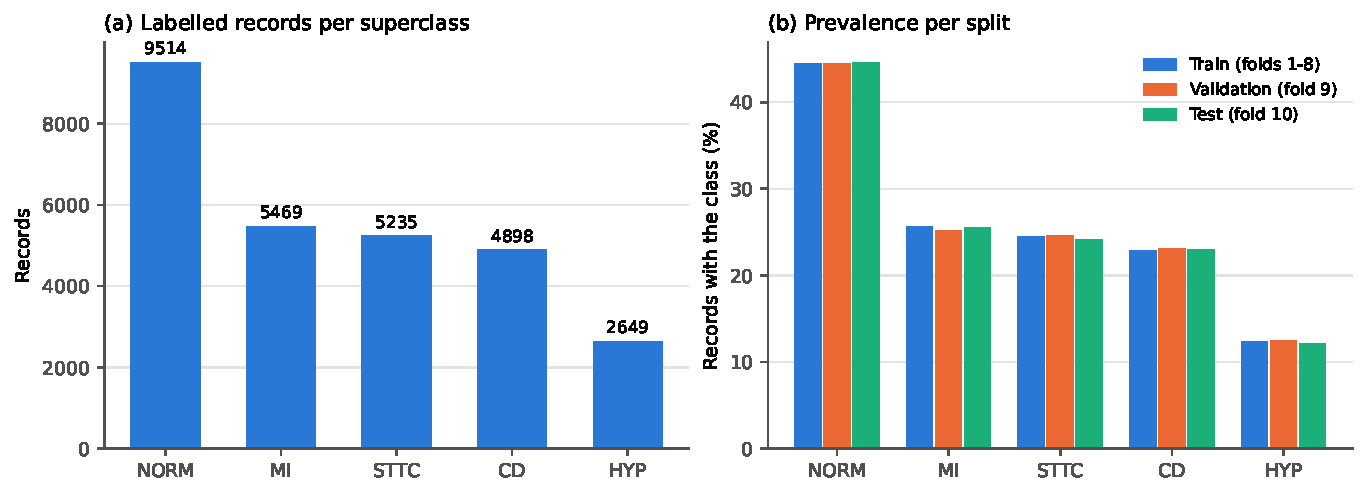
\includegraphics[width=\textwidth,height=0.42\textheight,keepaspectratio]{figures/eda_class_counts.pdf}
\caption[Records and prevalence per superclass and split]{PTB-XL superclasses. (a) Labelled records per superclass (a record may carry several). (b) Prevalence of each class in the training (folds 1--8), validation (fold 9) and test (fold 10) splits.}
\label{fig:eda_class_counts}
\end{figure}

% Shared float (common/make_floats.py). Figure: figures/eda_label_cooccurrence.pdf
\begin{figure}[htbp]
\centering
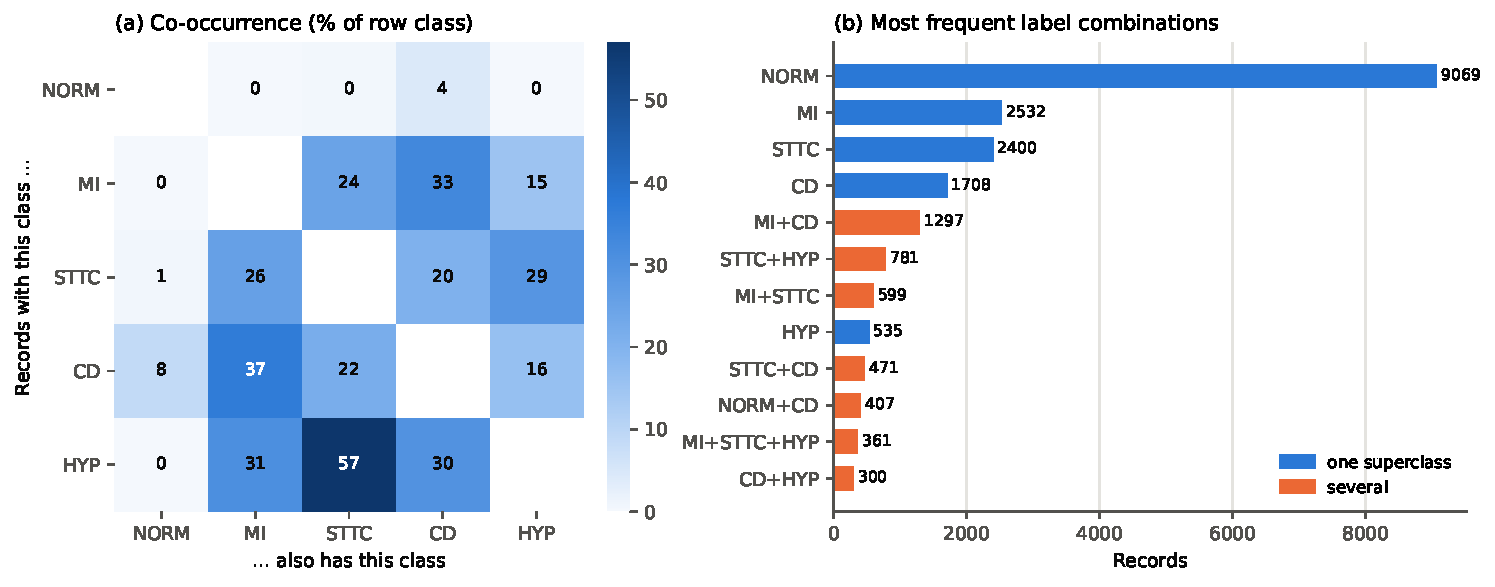
\includegraphics[width=\textwidth,height=0.42\textheight,keepaspectratio]{figures/eda_label_cooccurrence.pdf}
\caption[Co-occurrence and combinations of superclasses]{Multi-label structure. (a) Co-occurrence: percentage of the records of the row class that also carry the column class (not symmetric). (b) Most frequent label combinations; blue: one superclass, orange: several.}
\label{fig:eda_label_cooccurrence}
\end{figure}

% Shared float (common/make_floats.py). Figure: figures/eda_lead_stats.pdf
\begin{figure}[htbp]
\centering
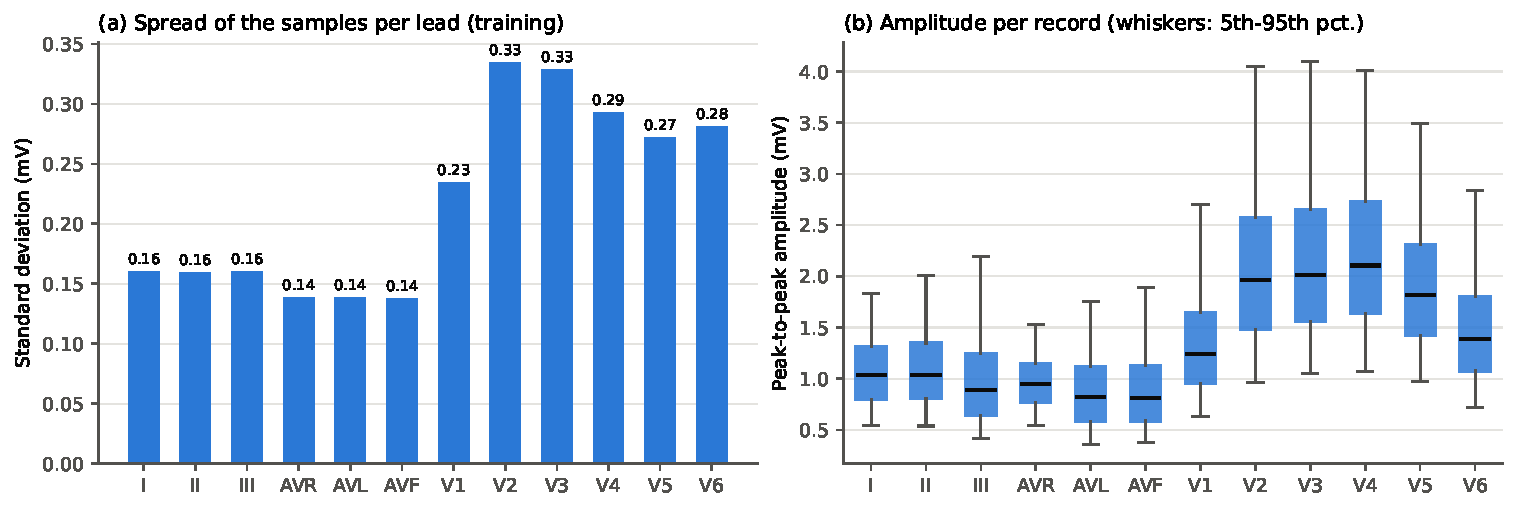
\includegraphics[width=\textwidth,height=0.42\textheight,keepaspectratio]{figures/eda_lead_stats.pdf}
\caption[Per-lead spread and amplitude]{Per-lead statistics of the training records. (a) Standard deviation of the samples (the values used by the per-lead z-score). (b) Peak-to-peak amplitude per record (box: quartiles; whiskers: 5th and 95th percentiles).}
\label{fig:eda_lead_stats}
\end{figure}


Figure~\ref{fig:eda_example_traces} shows lead II of one training record per superclass. The same
beat pattern repeats several times per record, at positions that differ from record to record, so a model
must recognise a pattern wherever it occurs in the ten seconds. This observation drives the comparison
of architectures in Section~\ref{sec:arch}.

% Shared float (common/make_floats.py). Figure: figures/eda_example_traces.pdf
\begin{figure}[htbp]
\centering
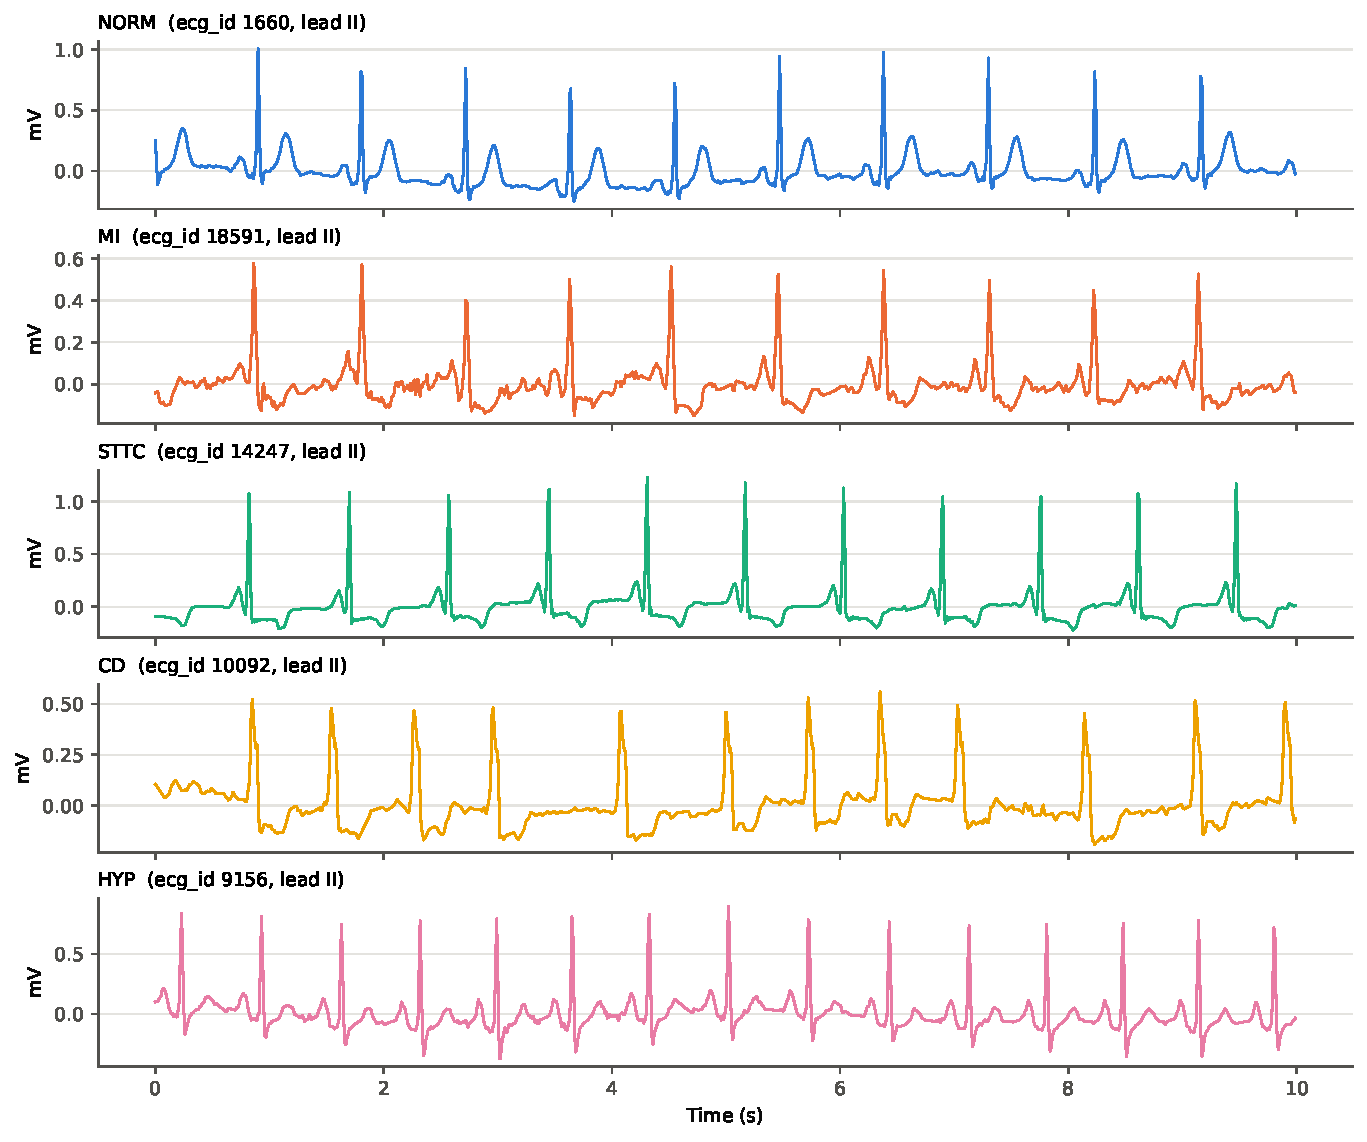
\includegraphics[width=\textwidth,height=0.42\textheight,keepaspectratio]{figures/eda_example_traces.pdf}
\caption[Lead II of one record per superclass]{Lead II of one training record per superclass (records with a single superclass, drawn at random with seed 42).}
\label{fig:eda_example_traces}
\end{figure}

